\subsection{Advanced Configuration and Power Interface (\gls{acpi})}
The ACPI Component Architecture (ACPICA) defines and implements a group of software
components that together create an implementation of the ACPI specification. A major goal of the
architecture is to isolate all operating system dependencies to a relatively small translation or
conversion layer (the OS Services Layer) so that the bulk of the ACPICA code is independent of
any individual operating system. Therefore, hosting the ACPICA code on new operating systems
requires no source changes within the ACPICA code itself.

The components of the architecture include:
\begin{itemize}
	\item An OS-independent, kernel-resident ACPICA Subsystem component that provides the fundamental ACPI services such as the AML interpreter and namespace management.
	\item An OS-dependent OS Services Layer for each host operating system to provide OS support for the OS-independent ACPICA Subsystem.
	\item An ASL compiler-disassembler for translating ASL code to AML byte code and for disassembling existing binary ACPI tables back to ASL source code.
	\item Several ACPI utilities for executing the interpreter in ring 3 user space, extracting binary ACPI tables from the output of the ACPI Dump utility, and translating the ACPICA source	code to Linux/Unix format.
\end{itemize}

In Figure \ref{fig:introduction-acpi-component-architecture}, the ACPICA subsystem is shown in relation to the host operating system, device driver, OSPM software, and the ACPI hardware

\begin{figure}[h]
	\centering
	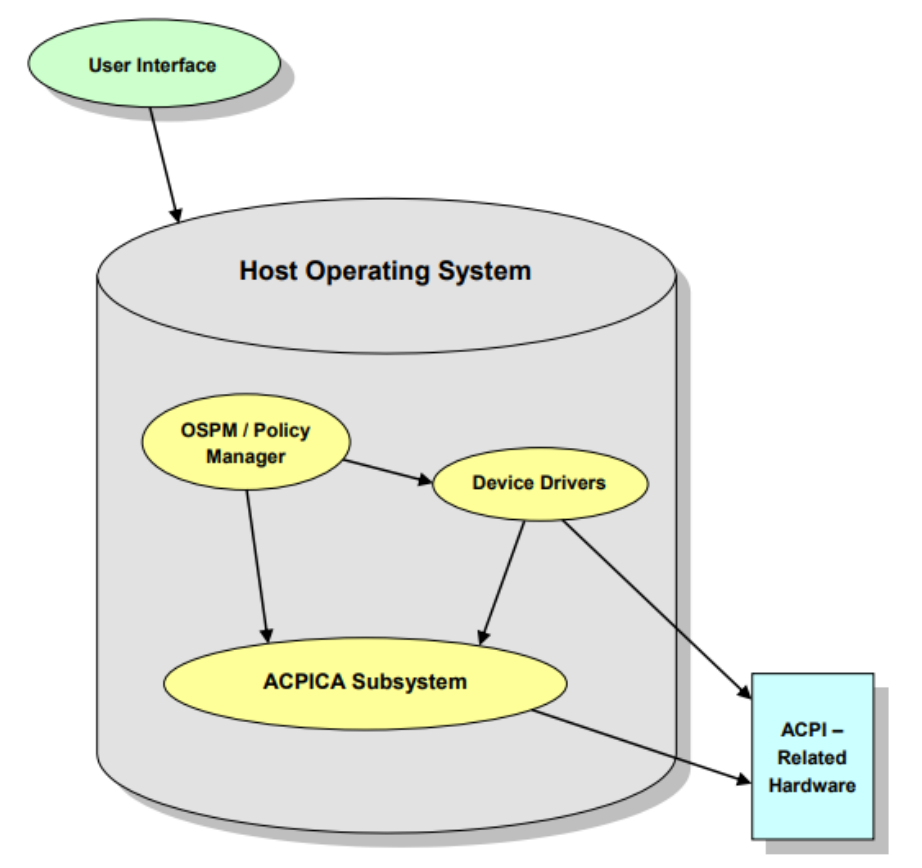
\includegraphics[width=0.7\linewidth]{introduction/acpi-component-architecture}
	\caption{The \gls{acpi} Component Architecture}\label{fig:introduction-acpi-component-architecture}
\end{figure}

\subsubsection{Overview of ACPICA Subsystem}
The ACPICA Subsystem implements the low level or fundamental aspects of the ACPI
specification. Included are an AML parser/interpreter, ACPI namespace management, ACPI table
and device support, and event handling. Since the ACPICA subsystem provides low-level system
services, it also requires low-level operating system services such as memory management,
synchronization, scheduling, and I/O.

To allow the ACPICA Subsystem to easily interface to any operating system that provides such
services, an Operating System Services Layer translates ACPICA-to-OS requests into the system
calls provided by the host operating system. The OS Services Layer is the only component of the
ACPICA that contains code that is specific to a host operating system.

Thus, the ACPICA Subsystem consists of two major software components:
\begin{itemize}
	\item The basic kernel-resident ACPICA Subsystem provides the fundamental ACPI services	that are independent of any particular operating system.
	\item The OS Services Layer (OSL) provides the conversion layer that interfaces the OS independent ACPICA Subsystem to a host operating system.
\end{itemize}

When combined into a single static or loadable software module such as a device driver or
kernel subsystem, these two major components form the ACPICA Subsystem. Throughout this
document, the term "ACPICA Subsystem" refers to the combination of the OS-independent
ACPICA Subsystem with an OS Services Layer components combined into a single module,
driver, or load unit.

\subsubsection{OS-independent ACPICA Subsystem}
The OS-independent ACPICA Subsystem supplies the major building blocks or subcomponents that are required for all ACPI implementations — including an AML interpreter, a namespace manager, ACPI event and resource management, and ACPI hardware support.

One of the goals of the ACPICA Subsystem is to provide an abstraction level high enough such
that the host operating system does not need to understand or know about the very low-level ACPI
details. For example, all AML code is hidden from the host. Also, the details of the ACPI hardware
are abstracted to higher-level software interfaces.

The ACPICA Subsystem implementation makes no assumptions about the host operating system or environment. The only way it can request operating system services is via interfaces provided by the OS Services Layer.

The primary user of the services provided by the ACPICA Subsystem are the host OS device drivers and power/thermal management software.

\subsubsection{Operating System Services Layer}
The OS Services Layer (or OSL) operates as a translation service for requests from the OS independent ACPICA subsystem back to the host OS. The OSL implements a generic set of OS service interfaces by using the primitives available from the host OS. Because of its nature.

The OS Services Layer must be implemented anew for each supported host operating
system. There is a single OS-independent ACPICA Subsystem, but there must be an OS Services
Layer for each operating system supported by the ACPI component architecture.

The primary function of the OSL in the ACPI Component Architecture is to be the small
glue layer that binds the much larger ACPICA Subsystem to the host operating system. Because
of the nature of ACPI itself — such as the requirement for an AML interpreter and management
of a large namespace data structure — most of the implementation of the ACPI specification is
independent of any operating system services. Therefore, the OS-independent ACPICA Subsystem
is the larger of the two components.

The overall ACPI Component Architecture in relation to the host operating system is Figure

\begin{figure}[h]
	\centering
	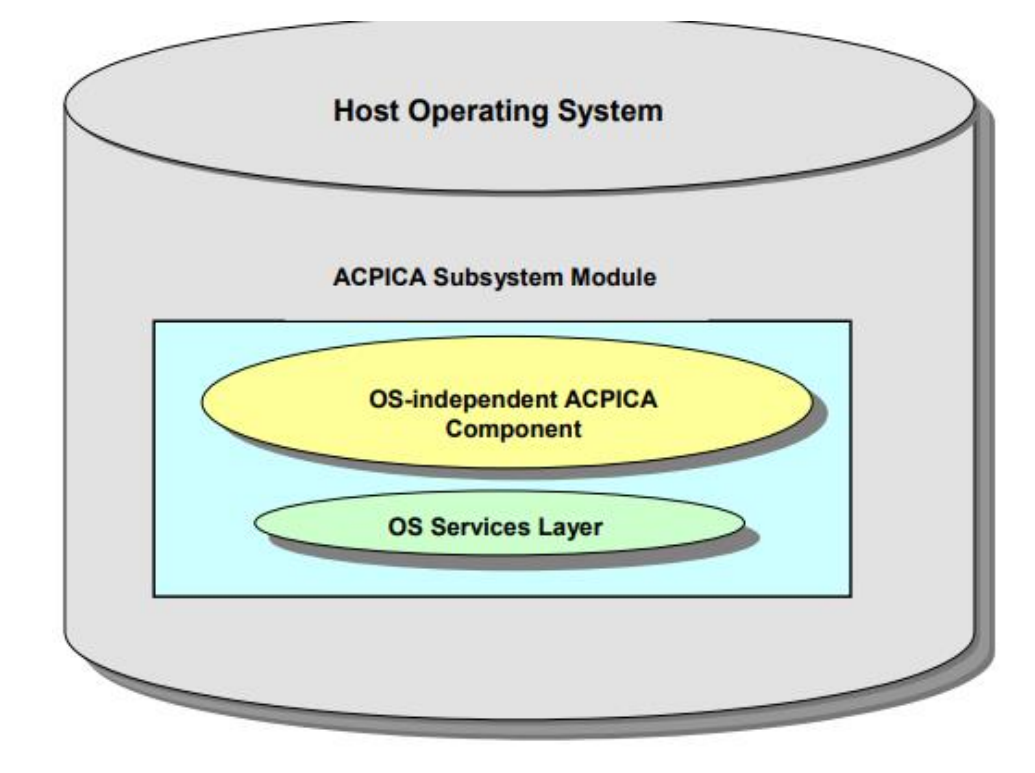
\includegraphics[width=0.7\linewidth]{introduction/acpica-subsystem-architecture}
	\caption{ACPICA Subsystem Architecture}\label{fig:introduction-acpica-subsystem-architecture}
\end{figure}

\subsubsection{ACPICA Subsystem Interaction}
The ACPICA Subsystem implements a set of external interfaces that can be directly called from
the host OS. These Acpi* interfaces provide the actual ACPI services for the host. When operating
system services are required during the servicing of an ACPI request, the Subsystem makes
requests to the host OS indirectly via the fixed AcpiOs* interfaces. The diagram below illustrates
the relationships and interaction between the various architectural elements by showing the flow
of control between them. Note that the OS-independent ACPICA Subsystem never calls the host directly instead it makes calls to the AcpiOs * interfaces in the OSL. This provides the ACPICA
code with OS-independence.

The Interaction between the Architectural Components is shown in Figure \ref{fig:-introduction-acpi-interaction-between-the-architectural-components}

\begin{figure}[h]
	\centering
	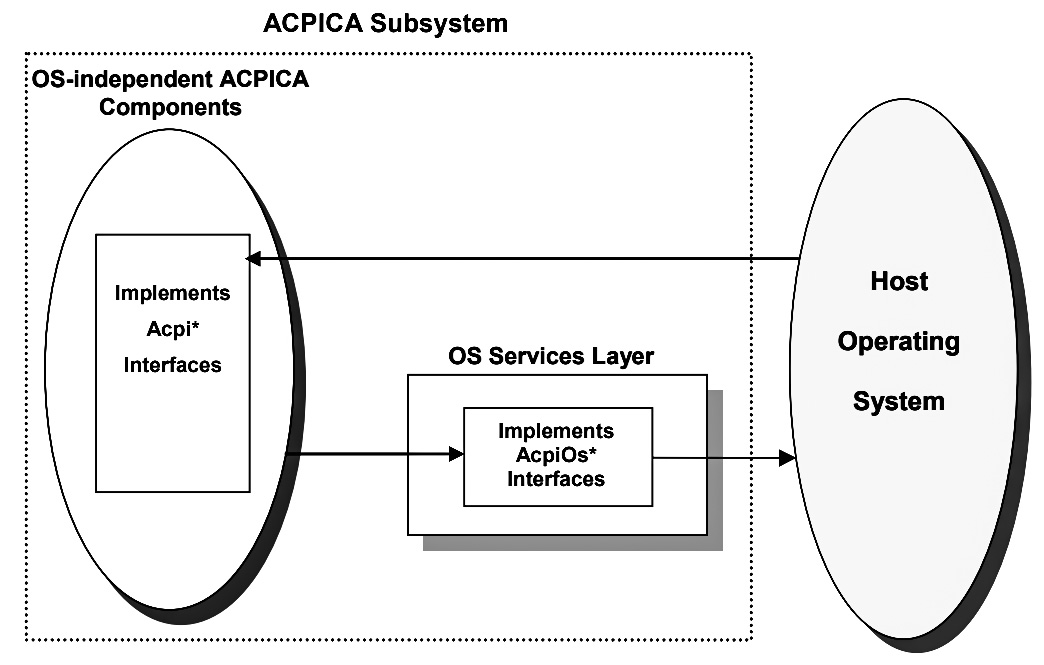
\includegraphics[width=0.7\linewidth]{introduction/acpi-interaction-between-the-architectural-components}
	\caption{Interaction between the Architectural Components}\label{fig:-introduction-acpi-interaction-between-the-architectural-components}
\end{figure}

